\section{\SecAdvanceBulkjob} \label{sec:bulkjob}
%====================================================================================

\scalerm には「一括実行機能」、いわゆるバルクジョブ機能が備わっている。
これは、パラメタスイープ実験、初期値アンサンブル実験や、
タイムスライス気候実験など多数の実験を行う場合に便利な機能である。
\scalerm モデル本体の実行はもちろん、ドメインネスティング実験の場合でも利用できるし、
地形・土地利用データ作成(地形コピーを利用しない場合のみ)、
初期値/境界値作成にも適用可能である。
%そして後処理ツールのnet2g(netcdf2grads\_bulkを使用)

\proofcomment{netcdf2grads\_bulkというコマンドがあるということでしょうか?}\\
\replycomment{今回のリリースにはnetcdf2grads\_bulkは含まれないので、netcdf2grads\_bulkに関する記述は削除しました。(足立)}

各プログラムの実行内容は異なっていても構わないが、
MPI並列としての構造は共通していなければならない点に注意すること。
1つの計算事例をここでは「ジョブ」と呼ぶこととする。
以下では、3つの2段オンライン・ネスティング実験を一括に行う例をもとに説明する
(積分期間、もしくは計算領域中心が異なっている3つのジョブを想定している)。


\begin{figure}[t]
\begin{center}
  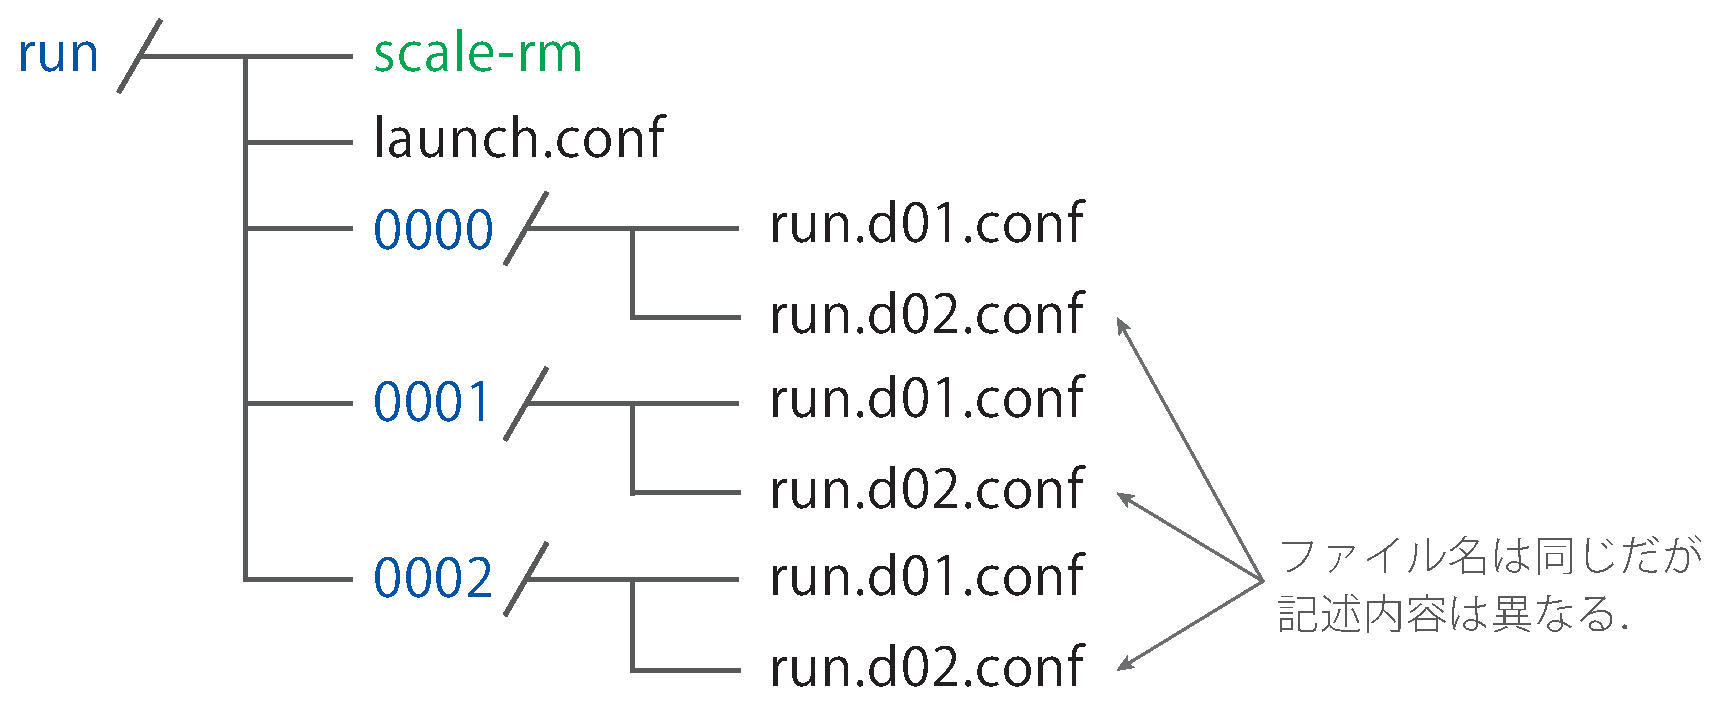
\includegraphics[width=0.6\hsize]{./figure/bulkjob_directory_structure.eps}\\
  \caption{バルクジョブ機能を使ってscale-rmを実行する場合のディレクトリ構造. ``0000''や``0001''はジョブ番号
           に対応する名前を持ったジョブディレクトリである。各ジョブディレクトリの中には、そこで実行する実験に関する
           設定ファイルが置かれている。データパラメタテーブルなどのファイルやディレクトリの記述は割愛しているが、
           それらも必要に応じて適切に配置する必要がある。}
  \label{fig_bulkjob}
\end{center}
\end{figure}

\proofcomment{図が、scale-lesになっています。scale-rmの間違いでしょうか?}


バルクジョブ実行するにあたって下記のものを事前に準備する必要がある。
\begin{itemize}
\item バルクジョブ用のディレクトリ構造
\item 実験に必要なすべての設定ファイル
\item 実験に必要なすべての外部入力データ
\end{itemize}

まず、図\ref{fig_bulkjob}に示すようなディレクトリ構造を準備する。``0000''や``0001''といったディレクトリは、
ジョブ番号に対応する名前を持ったジョブディレクトリである。ジョブディレクトリは必ず4桁の数字で、ジョブ番号はゼロから
数え上げられる。これらのディレクトリの中には設定ファイルが収められている。
今回は2段オンライン・ネスティング実験を想定しているので、``run.d01.conf''と``run.d02.conf''の2つのファイルが準備
されている。各ジョブディレクトリにある設定ファイルの名前は同じにする必要があるが、内容は異なっていても構わない。
ただし、\textcolor{red}{ドメイン毎に使用するMPIプロセス数は全てのジョブで共通していなければならない。}
設定ファイル内にバルクジョブ機能用に追加する設定項目はないが、\textcolor{red}{入出力ファイルのPATHを適切に
記述する}必要がある。以下にジョブ0000番のrun.d01.confの抜粋を示す。\\

\noindent {\small {\gt
\ovalbox{
\begin{tabularx}{140mm}{l}
\verb|&PARAM_IO| \\
\textcolor{blue}{\verb| IO_LOG_BASENAME = "0000/LOG_d01",|} \\
\verb|/| \\
 \\
\verb|&PARAM_RESTART| \\
\verb| RESTART_OUTPUT       = .true.,| \\
\textcolor{blue}{\verb| RESTART_OUT_BASENAME = "0000/restart_d01",|} \\
\textcolor{cyan}{\verb| RESTART_IN_BASENAME  = "../init/0000/init_d01_00013046400.000",|} \\
\verb|/| \\
 \\
\verb|&PARAM_TOPO| \\
\textcolor{cyan}{\verb| TOPO_IN_BASENAME = "../pp/0000/topo_d01",|} \\
\verb|/| \\
 \\
\verb|&PARAM_LANDUSE| \\
\textcolor{cyan}{\verb| LANDUSE_IN_BASENAME = "../pp/0000/landuse_d01",|} \\
\verb|/| \\
 \\
\verb|&PARAM_ATMOS_BOUNDARY| \\
\verb|     〜 中略 〜|\\
\textcolor{cyan}{\verb| ATMOS_BOUNDARY_IN_BASENAME    = "../init/0000/boundary_d01",|} \\
\verb|     〜 以下略 〜|\\
\verb|/| \\
 \\
\verb|&PARAM_HISTORY| \\
\textcolor{blue}{\verb| HISTORY_DEFAULT_BASENAME  = "0000/history_d01",|} \\
\verb|     〜 以下略 〜|\\
\verb|/| \\
\end{tabularx}
}}}\\

\noindent 上記の設定ファイルの設定例のうち、
青色文字の部分は出力ファイルの指定、
水色文字の部分は入力ファイルの指定である。
図\ref{fig_bulkjob}を見てわかるように、
実行バイナリ(scale-rm)があるのは``runディレクトリ''の下で、
ジョブディレクトリも実行バイナリと同じ階層にある。
従って、ジョブ0000番において、実行バイナリからみてデータを出力するべきディレクトリは、
``0000/''の下である。そこで出力ファイル名の指定として``0000/***''と記述している。

入力ファイルについても同様である。
ここでは、runディレクトリと同じ階層にppディレクトリやinitディレクトリがあり、
その中にまたジョブディレクトリが作成してあって、
それらの中に入力ファイルが保管されている状況を想定している。
従って、runディレクトリの下で実行される実行バイナリにとっては、``../pp/0000/***''といったPATHになる。

バルクジョブ機能は、オンライン・ネスティング実験で利用したMPIプロセスを分割・分配する機能を使って実装されている。
したがって、ジョブの起動のために``launch.conf''ファイルが必要になる。オンライン・ネスティング実験とバルクジョブ機能を
併用して実行する今回のような場合もlaunch.confファイルは1つだけで良い。\\

\noindent {\small {\gt
\ovalbox{
\begin{tabularx}{140mm}{l}
\verb|&PARAM_LAUNCHER| \\
\verb| NUM_BULKJOB = 3,| \\
\verb| NUM_DOMAIN  = 2,| \\
\verb| PRC_DOMAINS = 9,36,| \\
\verb| CONF_FILES  = run.d01.conf,run.d02.conf,| \\
\verb|/| \\
\end{tabularx}
}}}\\

\noindent 上記がオンライン・ネスティング実験とバルクジョブ機能を併用して実行する場合のlaunch.confファイルの中身である。
オンライン・ネスティング実験の場合のlaunch.confファイルに対して、\nmitem{NUM_BULKJOB}の設定項目を加えただけとなっている。
ここで実行するジョブ数は3つであるので、\nmitem{NUM_BULKJOB}に対して``3''と指定する。シングルドメイン実験として
バルクジョブ機能を利用する場合は、\nmitem{NUM_DOMAIN = 1}と指定して、\nmitem{CONF_FILES}に1つだけ設定ファイルを指定すればよい。
実行時のコマンドは、

\begin{verbatim}
 $ mpirun  -n  135  ./scale-rm  launch.conf
\end{verbatim}

となる。ここでは1ジョブあたり、$9 + 36 = 45$プロセス使用し、全体で3つのジョブを実行するので、総計で135プロセスを
必要とする。

実行すると得られるLOGファイルに、MPIプロセスを分割した時の情報が示されている。LOGファイルを開いて最初の
「SCALEロゴ」のあとに下記のようなメッセージが出力される。\\

\noindent {\small {\gt
\ovalbox{
\begin{tabularx}{140mm}{l}
\verb| ++++++ Start MPI| \\
\verb| *** UNIVERSAL_COMM_WORLD        :        0| \\
\verb| *** total process [UNIVERSAL]   :      135| \\
\verb| *** my process ID [UNIVERSAL]   :       36| \\
\verb| *** master rank?  [UNIVERSAL]   :        F| \\
\verb| *** GLOBAL_COMM_WORLD           :        3| \\
\verb| *** total process [GLOBAL]      :       45| \\
\verb| *** my process ID [GLOBAL]      :       36| \\
\verb| *** master rank?  [GLOBAL]      :        F| \\
\verb| *** LOCAL_COMM_WORLD            :        4| \\
\verb| *** total process [LOCAL]       :        9| \\
\verb| *** my process ID [LOCAL]       :        0| \\
\verb| *** master rank?  [LOCAL]       :        T| \\
\verb| *** ABORT_COMM_WORLD            :        0| \\
\verb| *** master rank ID [each world] :        0| \\

\end{tabularx}
}}}\\


\proofcomment{以下の記述、上の表とあっていますか?あってないように思います。総プロセス数は、135ではないの???何度何度も言っていますので、担当者へ確認をとられたと思いますし、合っているの化も知れませんが、私には理解不能でした。}

これらのうち、\verb|[LOCAL]|と表記されている項目はドメイン内のプロセスグループ、\verb|[GLOBAL]|と表記されている項目は
ネスティング・グループ、\verb|[UNIVERSAL]|と表記されて項目はジョブ・グループに関する情報である。
したがって、このLOGメッセージから、当該ドメインは12-MPI並列で実行されており、オンライン・ネスティング実験は総計で
48プロセス使用して実行され、バルクジョブ全体では1488プロセスが使用されているため、同時に31個のジョブが走っていたことがわかる。
異常終了したときにも、この表記法に従ってメッセージが出力されるので、これを理解しているとバルクジョブ機能を使って多量に
走らせている場合にも、どのプロセスがエラーを発生したのか即座に判断できる。ちなみに現在のバルクジョブ機能では、
1つのジョブがエラーを発生し、異常終了状態に入ると全てのジョブが異常終了する。



%%%%%%%%%%%%%%%%%%%%%%%%%%%%%%%%%%%%%%%%%%%%%%%%%%%%%%%%%%%%%%%%%%%%%%%%%%%%%%%%%%%%%%
